\documentclass[conference]{IEEEtran}
\ifCLASSINFOpdf
  \usepackage[pdftex]{graphicx}
  \graphicspath{{../pdf/}{../jpeg/}}
  \DeclareGraphicsExtensions{.pdf,.jpeg,.png}
\else
  \usepackage[dvips]{graphicx}
  \graphicspath{{../eps/}}
  \DeclareGraphicsExtensions{.eps}
\fi
\usepackage{cite}
\usepackage{times}
\usepackage[cmex10]{amsmath}
\usepackage{algorithmic}
\usepackage{array}
\usepackage[tight,footnotesize]{subfigure}
\usepackage{fixltx2e}
\usepackage{url}
\usepackage{lipsum}

\begin{document}

% paper title
\title{Iterative MIMO Detection for Large Wireless MIMO Systems}

% author names and affiliations
\author{
\IEEEauthorblockN{Alexandre P. J. Dixneuf}
\IEEEauthorblockA{Student, CentraleSupélec}
\and
\IEEEauthorblockN{Antoine Berthet}
\IEEEauthorblockA{Professor, CentraleSupélec}
}

% make the title area
\maketitle

\begin{abstract}
    This report explores iterative detection and decoding techniques for large-scale MIMO systems, focusing on the application of Belief Propagation (BP) and its Gaussian variant (GaBP) within factor graphs. Starting with a detailed derivation of message-passing equations, the study evaluates baseline performance under massive MIMO settings. A group-wise approximation strategy is then introduced to reduce computational complexity by modeling subsets of variables as Gaussian-distributed. The work further integrates Low-Density Parity-Check Codes (LDPCC) and Bit-Interleaved Coded Modulation (BICM) to enhance error correction and spectral efficiency. Through simulations and performance analysis, the proposed implementations demonstrate potential improvements in complexity-performance tradeoffs, paving the way for scalable receiver architectures suitable for next-generation wireless networks such as 5G and beyond.
\end{abstract}

% Found this command online to force wey
\providecommand{\keywords}[1]{\textbf{\textit{Index terms---}}#1}
\begin{keywords}
\textbf{Massive MIMO, Belief Propagation, Gaussian Approximation, Factor Graphs, LDPC Codes, BICM, Iterative Detection}
\end{keywords}

\IEEEpeerreviewmaketitle

\section{Introduction}
\lipsum[2]

\section{Background}
\lipsum[3]\cite{ExampleBIB}

\section{Theory and Reasoning}
\subsection{Theory}
\lipsum[5]

\subsection{Reasoing}
\lipsum[6]
\ref{fig:example}.
\begin{figure}[h!]
    \centering
    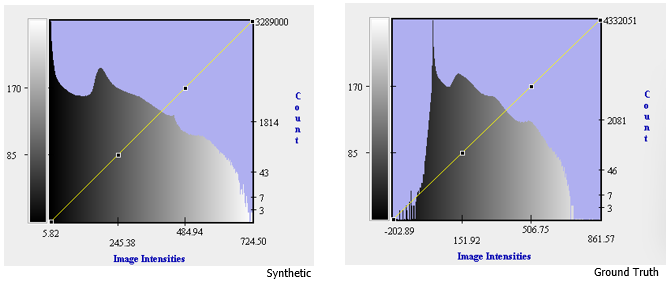
\includegraphics[width=0.30\textwidth]{Histogram Comparison.png}
    \caption{A side-by-side comparison of the intensity histogram between the post-processing synthesized T2w compared to the ground truth.}
    \label{fig:example}
\end{figure}

\section{Methods}
To run the necessary simulations, several criteria had to be met. To begin, an overall network simulation needed to be created. This simulation must handle the creation of a random signal, the propagation of the signal through a channel, and then the easy manipulation and handling of the necessary data and problem parameters. Then, a basic decoder is necessary to allow for easy addition of decoders. Since the average user will use completely different frameworks for any and all codes, the simulation uses a virtual class Decoder which handles most of the data. This allows new decoder classes to simply override the virtual decode function to properly run, and thus new decoders can be added in the future for proper comparison. Lastly, the individual decoders analyzed throughout this report were implemented.

\subsection{General Structure}
The simulation depends on the use of a storage class called ProblemParameters. The simulation of transmitted signals in a MIMO system depends on multiple variables, such as the number of transmitting antennas, receiving antennas, the degree of modulation, the number of time steps and/or the signal-to-noise ratio. The variables all have different constraints, including non-negativity and the modulation required to be a power of 4. To avoid constant checks to avoid errors and bugs, all of the data is stored in the storage class ProblemParameters. The class’s task is to verify the parameters given are acceptable and to convert everything to constants such that they may no longer be altered. It also keeps a constant structure so that every future component knows the proper steps to handle the data.
The next component is the class MySignal. This class is similar to the ProblemParameters in that it has the main purpose of being a robust storage class. Rather than trusting the user to know what format the signal should be, it forces a constant format, and verifies the accuracy and altering of the contained data. It also serves to generate the random signal, although it does mean it would require additional steps to run the simulation on given data rather than random data. While this will have no effect on the study’s result, it does hurt any future application of this code.
The next class is QAMConstellation. This class serves to independently handle the M-QAM modulation of signals, as well as receiving and drawing the proper gray code constellation.
Lastly, there remains the Channel class. This class handles taking the data, generating the channel conditions, and propagating the given signal through the channel.

\subsection{Virtual Decoder}
One of the guiding principles behind the structure of the code in this project is to ensure that future decoders can be easily added and thus compared to the current methods. To this purpose, a virtual Decoder class was developed. This class handles taking in any data that a decoder could use, all the while keeping the rest of the data still accessible in case of non-standard decoders. Then, it handles the majority of the work necessary for a C++ class. It leaves only the function "decode" virtual such that overriding classes only need to override the single function to be fully compatible. 

\subsection{Belief Propagation Decoder}

\subsection{Guassian Approximation Belief Propagation Decoder}

\subsection{Clustered (Group-Wise) Decoder}

\subsection{Low-Density Parity-Check Code Decoder}

\subsection{Bit Interleaved Constellation Modulation Decoder}

\section{Experiments and Results}
There are five indepenent variables being verified during this project: the number of transmitting antennas, the number of receiving antennas, the number of messages sent, the level of modulation (M-QAM), and the signal-to-noise ratio (SNR) of the transmitted signal. It would be impossible to test every combination of every variable to receive usable data, so a base framework was used. In "base" conditions, there are two transmitting and receiving antennas each, only two messages are sent in 16-QAM with an SNR of 20. Then, each variable indepently will be selected, going from a given minimum and maximum value while the ramaining vatiables are set to constant be the base conditions. To allows for direct comparison between each variable and the resulting accuracy of the decoders.

\subsection{Transmitting Antennas}
The transmitting antenna can be considered the most constraining variable, as most decoding methods were unablet to handle anything past 5 transmitting antennas. Therefore, the range of tested values was from 2 antennas to 5 antennas, enough to get a general understanding of the relation between the number of antennas and the overall accuracy, without spending several days per simulation.

\subsection{Receiving Antennas}
The receiving antennas were must less constraining than the receiving antennas, and thus a larger range of 2 to 10 antennas was able to be used.

\subsection{Messages Sent}
Compared to the previous sections, the number of messages sent has very little effect on the overall complexity of the decoders. Instead, it only lengthened the length of the simulations. A larger range of values was therefore possible, and thus the minimum of 2 and maximum of 20 was used.

\subsection{M-Modulation}
Testing values of M-QAM modulation was complicated, as only square constellations were possible to test, meaning values go from 4, to 16, then 64, 256, and then 1024. This means only 5 simulations change the complexity of the simulation by a factor of almost 1000. 1024 was too complicated and 4 gave no information as even a guess could have good decoding odds, so the values of 16-QAM, 64-QAM, and 256-QAM were used. While this gives minimal data, it should still give a rough idea of the relation.

\subsection{Signal-to-Noise Ratio}
The SNR has no effect on the complexity of the system, so a large range of 10 to 40 was able to be used.

\section{Discussion}
\lipsum[10]

% References
\begin{thebibliography}{1}
\bibitem{ExampleBIB}
Gruszecki M, Lancaster G, Stefanovska A, Neary JP, Dech RT, Guminski W, Frydrychowski AF, Kot J, Winklewski PJ. \emph{Human Subarachnoid Space Width Oscillations in the Resting State}, 2018
\end{thebibliography}
\end{document}